%! Author = wolfram_e_laube
%! Date = 06.05.24

\item[(a)]
\subsection{Task (a): Real and Imaginary Parts of $X(f)$}

\subsection{Problem Statement}
The task involves analyzing the spectrum $X(f)$ of an analog signal $x(t)$, where the spectrum's magnitude and phase are given by specific mathematical functions. The goal is to draw and interpret the real and imaginary parts of the spectrum $X(f)$ based on these definitions.

\subsection{Analysis}
\subsubsection{Spectrum Definitions}
The spectrum of the signal is defined in terms of its magnitude $|X(f)|$ and phase $\phi_x(f)$ as follows:
\begin{itemize}
    \item \textbf{Magnitude $|X(f)|$:}
    \[
    |X(f)| =
    \begin{cases}
    A & \text{for } -5 \leq f \leq -1 \text{ and } 1 \leq f \leq 5 \\
    -Af & \text{for } -1 \leq f < 0 \\
    Af & \text{for } 0 \leq f < 1 \\
    0 & \text{otherwise}
    \end{cases}
    \]
    \item \textbf{Phase $\phi_x(f)$:}
    \[
    \phi_x(f) =
    \begin{cases}
    \frac{\pi}{2} & \text{if } f < 0 \\
    -\frac{\pi}{2} & \text{if } f > 0 \\
    0 & \text{if } |f| > 5
    \end{cases}
    \]
\end{itemize}
These functions delineate a filter-like response, manipulating the amplitude of the signal across various frequency ranges, accentuating or attenuating frequencies based on the system's design.

\subsubsection{Computational Analysis}
Using Python with libraries such as NumPy and Matplotlib, the real $\text{Re}\{X(f)\}$ and imaginary $\text{Im}\{X(f)\}$ parts of the spectrum were computed based on the defined magnitude and phase. These parts were then visualized to provide insight into the distribution of the signal's spectral characteristics across the frequency spectrum.

\subsection{Conclusion}
The plots of the real and imaginary parts illustrate how the signal's spectrum is influenced by its magnitude and phase characteristics:
\begin{itemize}
    \item The \textbf{real part} is significant mainly near zero, reflecting the brief non-zero contributions of $\cos(\phi_x(f))$ as it passes through zero at $f = 0$.
    \item The \textbf{imaginary part} demonstrates variable contributions, capturing the essence of the magnitude changes across the specified frequency ranges, showing the system's handling of different frequency components.
\end{itemize}

\begin{figure}[h]
    \centering
    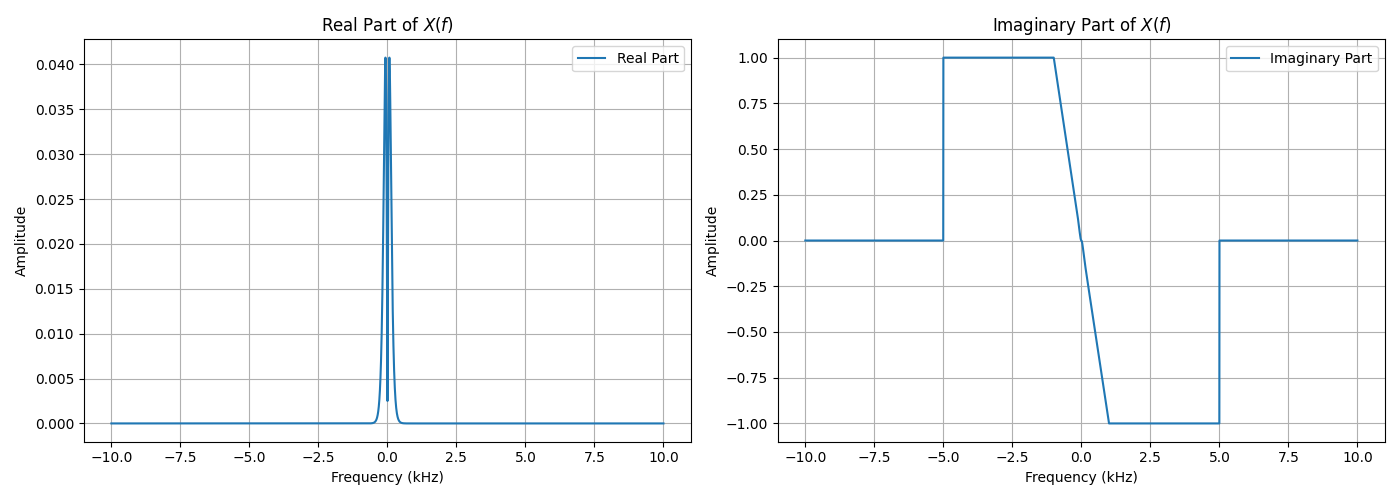
\includegraphics[width=0.49\textwidth]{fig/ex2_a_plot}
    \caption{Real and Imaginary Parts of $X(f)$}
    \label{fig:ex2_a_plot}
\end{figure}
